\documentclass[PredictiveAnalytics101.tex]{subfiles} 
\begin{document} 
% PLAN FOR SECTION
% ------------------------------------
% Confusion Matrix
% Accuracy Precision Recall
% F-measures
% Cost of MisClassification
% True Positive Rate
% Specificity and Sensitivitiy

% Re-writing a section from a shitty PACKT book
%============================%
\begin{frame}
\frametitle{Confusion Matrix}

\end{frame}
%================================

%==================================%
\begin{frame}
\frametitle{The Confusion Matrix}
The confusion matrix indicates that there were four true negative predictions, three
true positive predictions, two false negative predictions, and one false positive
prediction. Confusion matrices become more useful in multi-class problems, in
which it can be difficult to determine the most frequent types of errors.
\end{frame}
%==================================%
\begin{frame}
\textbf{Accuracy}\\
Accuracy measures a fraction of the classifier's predictions that are correct.
\end{frame}
%==================================%
\begin{frame}
	\textbf{Accuracy}\\
However, accuracy is not an informative metric if the proportions of
the classes are skewed in the population. For example, a classifier that predicts
whether or not credit card transactions are fraudulent may be more sensitive to
false negatives than to false positives. To promote customer satisfaction, the credit
card company may prefer to risk verifying legitimate transactions than risk ignoring
a fraudulent transaction. 
\end{frame}
%==================================%
\begin{frame}
\textbf{Accuracy}\\
Because most transactions are legitimate, accuracy is
not an appropriate metric for this problem. A classifier that always predicts that
transactions are legitimate could have a high accuracy score, but would not be
useful. For these reasons, classifiers are often evaluated using two additional
measures called precision and recall.
\end{frame}
%=================================%
\begin{frame}
\textbf{Precision and Recall}\\
Recall from Chapter 1, The Fundamentals of Machine Learning, that precision is the
fraction of positive predictions that are correct. For instance, in our SMS spam
classifier, precision is the fraction of messages classified as spam that are actually
spam. Precision is given by the following ratio:
\[ P = \frac{TP}{TP + FP} \]
\end{frame}
%=================================%
\begin{frame}
	\textbf{Recall}
\begin{itemize}
\item  called sensitivity in medical domains, recall is the fraction of the truly
positive instances that the classifier recognizes. A recall score of one indicates
that the classifier did not make any false negative predictions. 

\item For our SMS spam
classifier, recall is the fraction of spam messages that were truly classified as spam.
Recall is calculated with the following ratio:
\end{itemize}

\begin{figure}
\centering
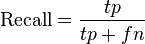
\includegraphics[width=0.7\linewidth]{recall}

\end{figure}

\end{frame}
%=================================%
\begin{frame}
\frametitle{Precision and Recall}
\begin{itemize}
\item Individually, precision and recall are seldom informative; they are both incomplete
views of a classifier's performance. 
\item Both precision and recall can fail to distinguish
classifiers that perform well from certain types of classifiers that perform poorly.
\item A
trivial classifier could easily achieve a perfect recall score by predicting positive for
every instance.
\end{itemize}
 
\end{frame}
%=================================%
\begin{frame}
\frametitle{Precision and Recall}
\begin{itemize}
\item For example, assume that a test set contains ten positive examples
and ten negative examples.
\item A classifier that predicts positive for every example will
achieve a recall of one, as follows:
\end{itemize}

10 1
10 0
R = =
+
\end{frame}
%=================================%
\begin{frame}
	
	\begin{itemize}
\item A classifier that predicts negative for every example, or that makes only false positive
and true negative predictions, will achieve a recall score of zero. 
\item Similarly, a classifier
that predicts that only a single instance is positive and happens to be correct will
achieve perfect precision.
	\end{itemize}

\end{frame}
%=================================%
\end{document}
